%%%%%%%%%%%%%%%%%%%%%%%%%%%%%%%%%%%%%%%%%
% Beamer Presentation
% LaTeX Template
% Version 1.0 (10/11/12)
%
% This template has been downloaded from:
% http://www.LaTeXTemplates.com
%
% License:
% CC BY-NC-SA 3.0 (http://creativecommons.org/licenses/by-nc-sa/3.0/)
%
%%%%%%%%%%%%%%%%%%%%%%%%%%%%%%%%%%%%%%%%%

%----------------------------------------------------------------------------------------
%	PACKAGES AND THEMES
%----------------------------------------------------------------------------------------

\documentclass{beamer}

\mode<presentation> {

% The Beamer class comes with a number of default slide themes
% which change the colors and layouts of slides. Below this is a list
% of all the themes, uncomment each in turn to see what they look like.

%\usetheme{default}
%\usetheme{AnnArbor}
%\usetheme{Antibes}
%\usetheme{Bergen}
%\usetheme{Berkeley}
%\usetheme{Berlin}
%\usetheme{Boadilla}
%\usetheme{CambridgeUS}
%\usetheme{Copenhagen}
%\usetheme{Darmstadt}
%\usetheme{Dresden}
%\usetheme{Frankfurt}
%\usetheme{Goettingen}
%\usetheme{Hannover}
%\usetheme{Ilmenau}
%\usetheme{JuanLesPins}
%\usetheme{Luebeck}
\usetheme{Madrid}
\usepackage[utf8]{inputenc}
\usepackage[brazilian]{babel}
%\usetheme{Malmoe}
%\usetheme{Marburg}
%\usetheme{Montpellier}
%\usetheme{PaloAlto}
%\usetheme{Pittsburgh}
%\usetheme{Rochester}
%\usetheme{Singapore}
%\usetheme{Szeged}
%\usetheme{Warsaw}

% As well as themes, the Beamer class has a number of color themes
% for any slide theme. Uncomment each of these in turn to see how it
% changes the colors of your current slide theme.

%\usecolortheme{albatross}
%\usecolortheme{beaver}
%\usecolortheme{beetle}
%\usecolortheme{crane}
%\usecolortheme{dolphin}
%\usecolortheme{dove}
%\usecolortheme{fly}
%\usecolortheme{lily}
%\usecolortheme{orchid}
%\usecolortheme{rose}
%\usecolortheme{seagull}
%\usecolortheme{seahorse}
%\usecolortheme{whale}
%\usecolortheme{wolverine}


%\setbeamertemplate{footline} % To remove the footer line in all slides uncomment this line
%\setbeamertemplate{footline}[page number] % To replace the footer line in all slides with a simple slide count uncomment this line

%\setbeamertemplate{navigation symbols}{} % To remove the navigation symbols from the bottom of all slides uncomment this line
}

\usepackage{subfig}
\usepackage{multirow}
\usepackage{hyperref}
\usepackage{graphicx} % Allows including images
\usepackage{booktabs} % Allows the use of \toprule, \midrule and \bottomrule in tables

%----------------------------------------------------------------------------------------
%	TITLE PAGE
%----------------------------------------------------------------------------------------

\title[Defesa de Mestrado]{Análise Digital de Imagens Microtomográficas de \\[0.1cm] Amostras de Reservatórios de Petróleo } % The short title appears at the bottom of every slide, the full title is only on the title page

\author[UNICAMP]{Candidata: Letícia da Silva Bomfim \\ Orientador: Prof. Dr. Hélio Pedrini \\Coorientador: Dr. Guilherme Avansi} % Your name
\institute[]{Universidade Estadual de Campinas \\ Instituto de Computação}
\subtitle{Defesa de Mestrado}
\medskip
%textit{.com} % Your email address

\date{20 de Fevereiro de 2020} % Date, can be changed to a custom date

\titlegraphic{
    \vspace{1cm}
    \hspace{10cm}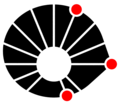
\includegraphics[width=1cm]{fig/logo-unicamp.png}
    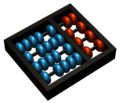
\includegraphics[width=1cm]{fig/logo-ic-unicamp.png}
}

\begin{document}

\begin{frame}
\titlepage % Print the title page as the first slide
\end{frame}

\begin{frame}
\frametitle{Índice} % Table of contents slide, comment this block out to remove it
\tableofcontents % Throughout your presentation, if you choose to use \section{} and \subsection{} commands, these will automatically be printed on this slide as an overview of your presentation
\end{frame}

%----------------------------------------------------------------------------------------
%	PRESENTATION SLIDES
%----------------------------------------------------------------------------------------

%------------------------------------------------
\section{Introdução} % Sections can be created in order to organize your presentation into discrete blocks, all sections and subsections are automatically printed in the table of contents as an overview of the talk
%------------------------------------------------
\subsection{Caracterização do Problema} 
\subsection{Implicação da Análise Digital}



\begin{frame}{Introdução}{Caracterização do Problema}
\begin{itemize}

\item Necessidade da identificação de um reservatório em potencial e auxílio no processo de tomada de decisão.

\item Uma análise prévia do campo de petróleo pode reduzir os gastos de um projeto e direcionam o seu gerenciamento. 

\item Aplicar análise digital substituindo o método de análise manual.
\begin{itemize}
\item Métodos destrutivos: expansão de gás hélio, injeção de nitrogênio..
\item \textbf{Métodos não destrutivos: análise digital}
\end{itemize}
\end{itemize}

\end{frame}



\begin{frame}{Introdução}{Implicação da Análise Digital}

\begin{itemize}
    \item Preservação das Rochas
    \item Análise profunda e minimalista das estruturas internas.
    
\end{itemize}

\begin{figure}[!htb]
\centering
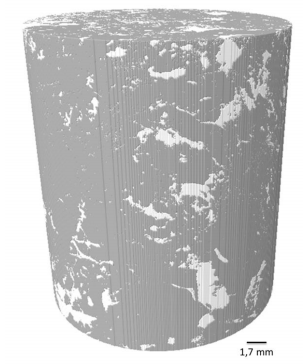
\includegraphics[width=2.5cm]{fig/amostra3d} \\
{\scriptsize Reprsentação digital de uma amostra de rocha.\protect\footnote{Piloto et al. Análise de Imagens de Micro-tomógrafo Digitalizadas para a Caracterização Microestrutural de Carbonatos. 2014}}
\end{figure}

\end{frame}


\begin{frame}{Introdução}{Como é feito este processo?}
    \begin{itemize}
        \item Sondagens e amostragens feitas dos campos em análise.
        \begin{itemize}
            \item O reservatório de petróleo ou zona de produção é uma formação rochosa permeável, porosa ou fraturada.~\protect\footnote{J. E. Thomas. Fundamentos de Engenharia de Petróleo. Interciência, 2001.}
        \end{itemize}
    \end{itemize}
    
    \begin{figure}[!htb]
        \centering
        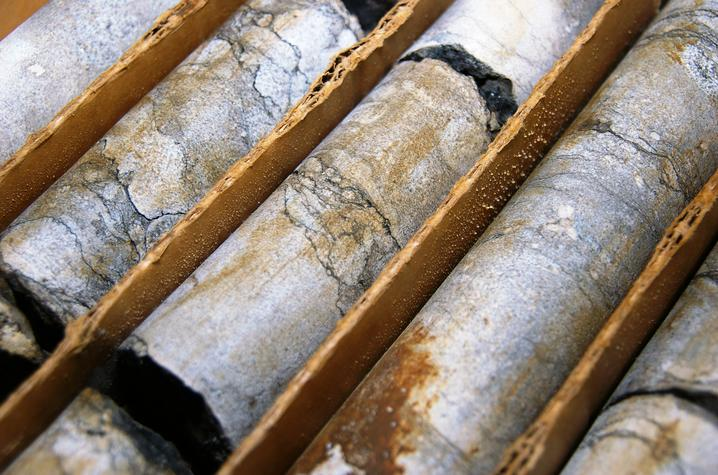
\includegraphics[width=6.5cm]{fig/testemunho.jpg}\\
        {\scriptsize Exemplo de testemunhos rochosos resultantes de sondagens. \protect\footnote{https://uknow.uky.edu/research/federal-grant-will-improve-rock-sample-archives-kentucky-geological-survey}}
    \end{figure}
\end{frame}

\begin{frame}{Introdução}{Aquisição das imagens}
    \begin{itemize}
        \item Técnica de Microtomografia
    \end{itemize}
    
    \begin{figure}[!htb]
        \centering
        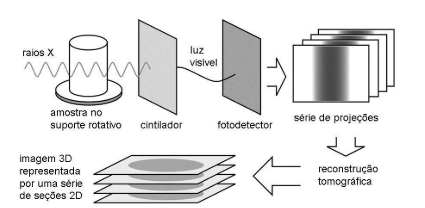
\includegraphics[width=8.5cm]{fig/metodoMRX.PNG}\\
        \scriptsize{Ilustração do processo de aquisição e reconstrução de imagens por tomografia computadorizada~\protect\footnote{D. Uliana, H. Kahn, R. Contessotto, and J. L. Antoniassi. Microtomografia de AltaResolução no Setor Mineral.HOLOS, 3:11–19, 2014}.}
        \label{fig:metodoMRX}
    \end{figure}
\end{frame}

\begin{frame}{Introdução}{Objetivos}

Produzir uma ferramenta que possibilite a geração de dados a respeito das estruturas internas à rochas, através da análise das imagens de MicroCT. Para isso, precisamos realizar:

    \begin{itemize}
        \item Levantamento bibliográfico e estudo das principais técnicas para análise digital dearenitos derivadas de imagens de microtomografia
        \item Extração das estruturas presentes na amostra a partir de uma técnica aprimorada de segmentação
        \item Classificação dos poros e fraturas a partir de suas características morfológicas
    \end{itemize}
    
\end{frame}

\begin{frame}{Introdução}{Hipóteses}
    \begin{itemize}
    
    \item A segmentação por limiarização é suficiente para extrair corretamente as estruturas internas das amostras?
    
    \item Quais as principais características a respeito da geometria das fraturas? É possível caracterizá-las a partir das estruturas extraídas?
    
    \item Qual a melhor maneira de interagir com os resultados obtidos pela caracterização?
    
    \end{itemize}
\end{frame}



\begin{frame}{Contextualização}
    \begin{itemize}
        \item \textbf{Poros}
        \begin{itemize}
            \item Representados por espaços vazios que dependem da forma, arranjo, variação e tamanho dos grãos presentes na rocha.
        \end{itemize}
        \item \textbf{Fraturas}
        \begin{itemize}
            \item Planos ao longo dos quais o estresse causou perda parcial de coesão na rocha.
        \end{itemize}
    \end{itemize}
    
    
    \begin{figure}[!htb]
        \centering
        \subfloat[]{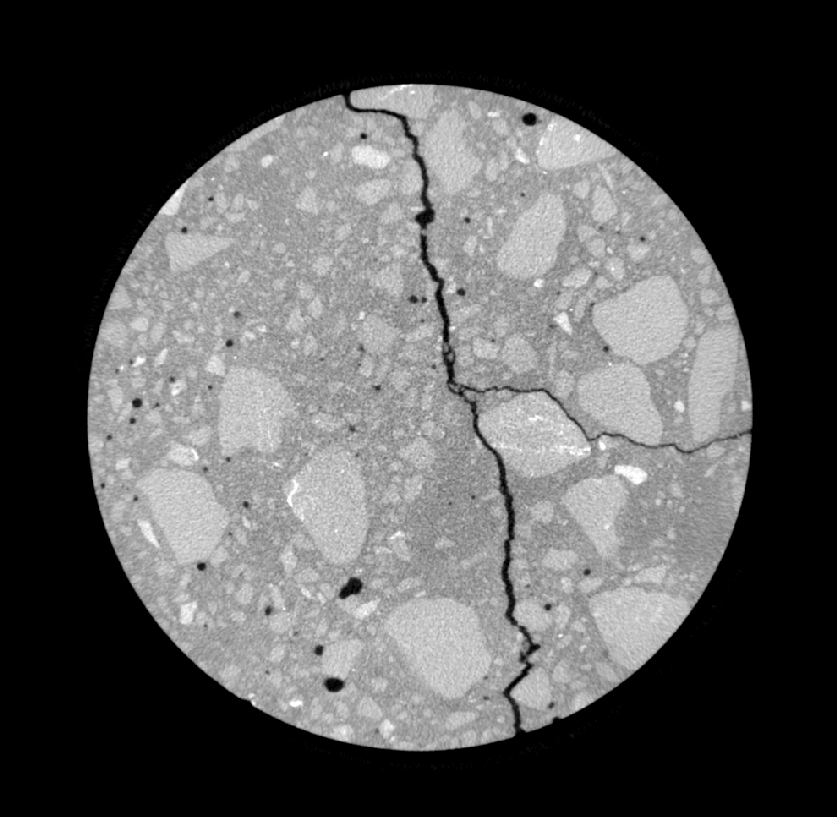
\includegraphics[height=3.0cm]{fig/fratura.png}} \hspace*{0.1cm}
        \subfloat[]{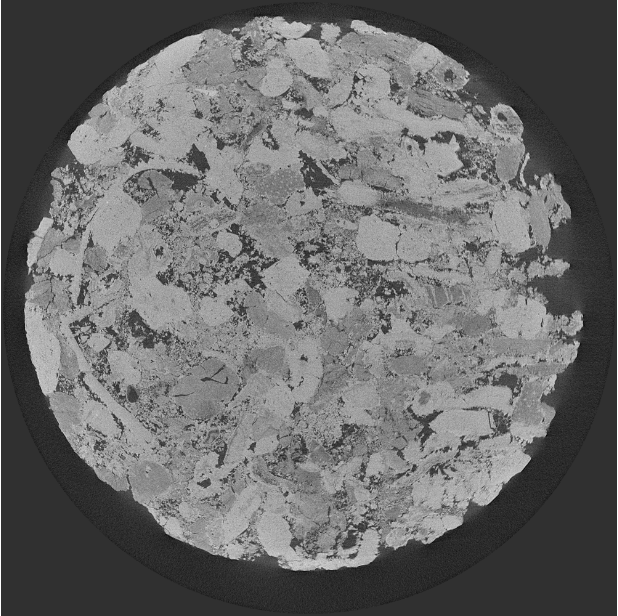
\includegraphics[height=3.0cm]{fig/img_original.png}}\\
         \scriptsize{Exemplos de imagens tomográficas. (a) imagem de rocha carbonática com a presença de uma fratura;~\protect\footnote{A.  du  Plasis.    Concrete  Cracking. 2014} (b) imagem de rocha apenas com poros.~\protect\footnote{T. Bultreys.  Estaillades Carbonate 2, 2016}.}
        \label{fig:microct}
    \end{figure}

\end{frame}

\begin{frame}{Contextualização}{Característica das Estruturas}
   As características permitem a existência do fluxo de fluídos, o que se encontra diretamente ligado a produtividade e lucratividade do reservatório. Algumas delas são:
   
    \begin{table}[]
        \begin{tabular}{c|c}
       \textbf{Poros}         &  \textbf{Fraturas}      \\ \hline
        Porosidade            & Tamanho       \\
        Circularidade         & Conectividade \\
        Visibilidade          & Densidade     \\
        \multicolumn{1}{l|}{} & Orientação   
        \end{tabular}
    \end{table}
\end{frame}

\begin{frame}{Materiais}{Base de Dados}
    \begin{itemize}
        \item \textit{Digital Rocks Portal}: Um repositório que promove um ambiente de recuperação, armazenamento, compartilhamento, organização e análise de imagens de microestruturas porosas variadas.
        \item Imagens com formato \texttt{.tiff} para facilitar a manipulação dos dados em 2D.
        \item Amostra milimétrica gerando imagens de alta resolução. 
    \end{itemize}
    
\end{frame}

\begin{frame}{Materiais}{Recursos Computacionais}
  \begin{itemize}
      \item \textbf{Principais Ferramentas:}
  \end{itemize}  
    \begin{figure}[!htb]
        \centering
        \subfloat[]{
\includegraphics[height=2cm]{fig/python.png}} \hspace*{0.3cm}
        \subfloat[]{
\includegraphics[height=2.0cm]{fig/opencv.png}}
        \hspace*{0.3cm}
        \subfloat[]{
\includegraphics[height=2.0cm]{fig/VTKlogo.png}} \hspace*{0.3cm}
        \subfloat[]{
\includegraphics[height=2.0cm]{fig/qt-creator-logo.png}} \hspace*{0.3cm}
        \\
         \scriptsize{Ferramentas utilizadas na construção da análise das imagens. (a) Python~\protect\footnote{https://www.python.org/} (b) OpenCV~\protect\footnote{https://opencv.org/} (c) Visualization Toolkit~\protect\footnote{https://vtk.org/} (d) QT Designer~\protect\footnote{https://qt.io/}}
        
    \end{figure}
\end{frame}

\begin{frame}{Metodologia}
    \begin{itemize}
        \item Fluxo da metodologia da ferramenta:
    \end{itemize}
    
     \begin{figure}[!htb]
        \centering
        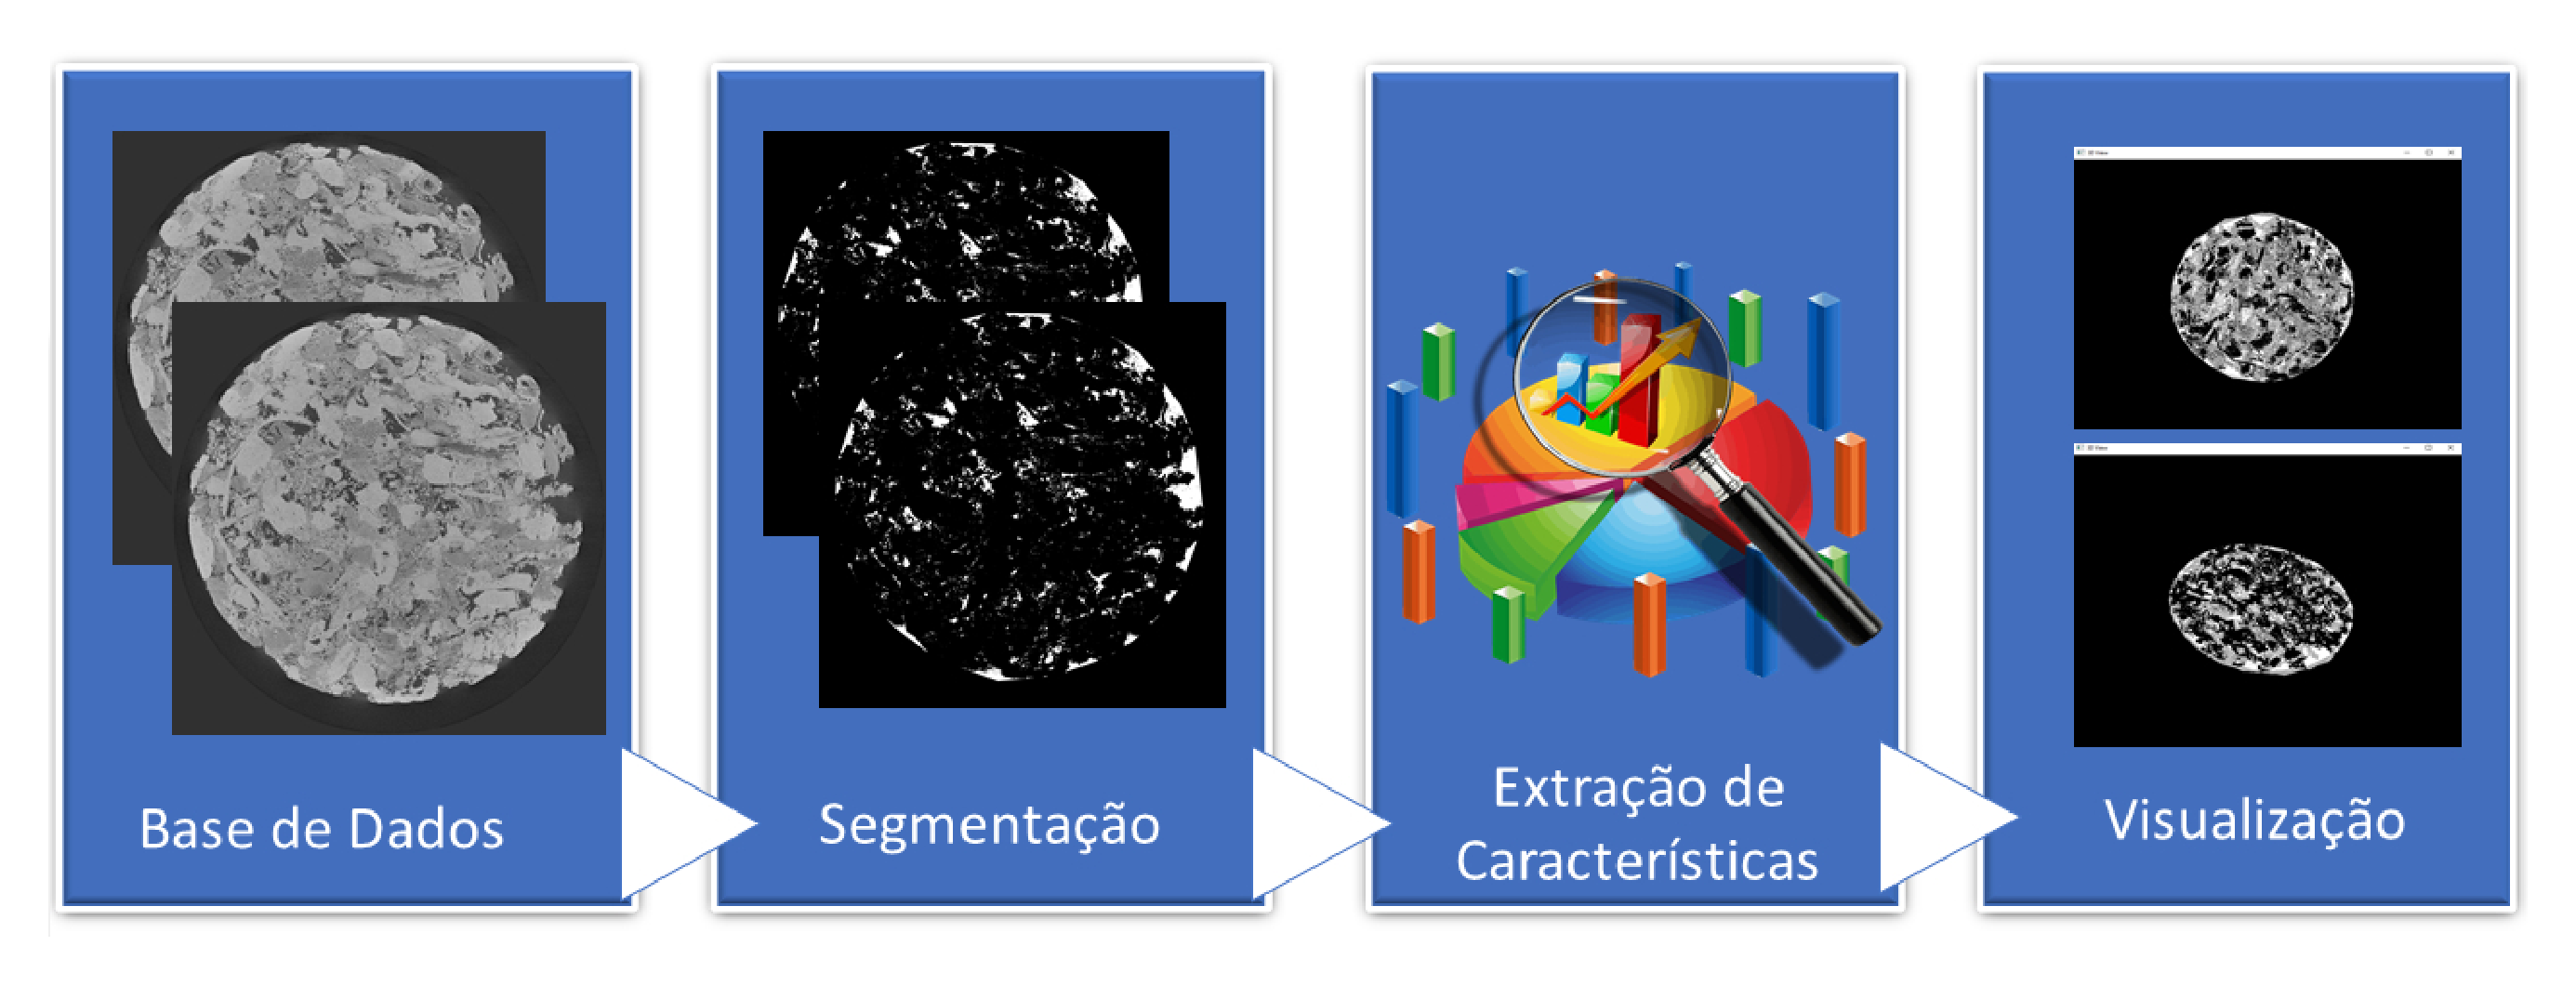
\includegraphics[width=12cm]{fig/descricao.pdf}\\
        \scriptsize{Diagrama da metodologia para análise de estruturas de rochas.}
        \label{fig:metodoMRX}
    \end{figure}
\end{frame}

\begin{frame}{Metodologia}{Segmentação}
 A segmentação é dividade em dois passos:
 \begin{itemize}
     \item A extração da região de interesse.
     \begin{itemize}
        \item Segmentação utilizando principalmente o método de \textit{Watershed}.
        \item Necessidade da aplicação série de técnicas de processamento de imagens. 
    \end{itemize}
    
     \item A extração das estruturas contidas na região de interesse.
     \begin{itemize}
         \item Segmentação utilizando o limiar de Otsu.
         \item Duas análises diferentes: \textbf{Poros e Fraturas}.
     \end{itemize}
 \end{itemize}

\begin{figure}[!htb]
        \centering
        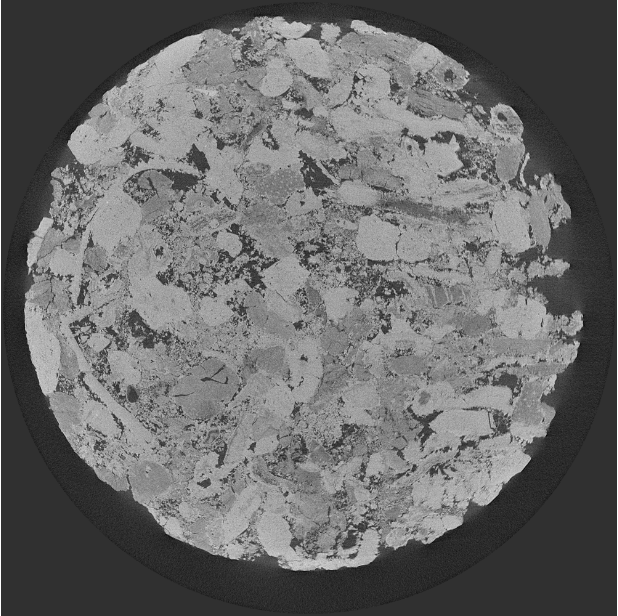
\includegraphics[width=3cm]{fig/img_original.png}
        
\includegraphics[width=3cm]{fig/mask.png}
        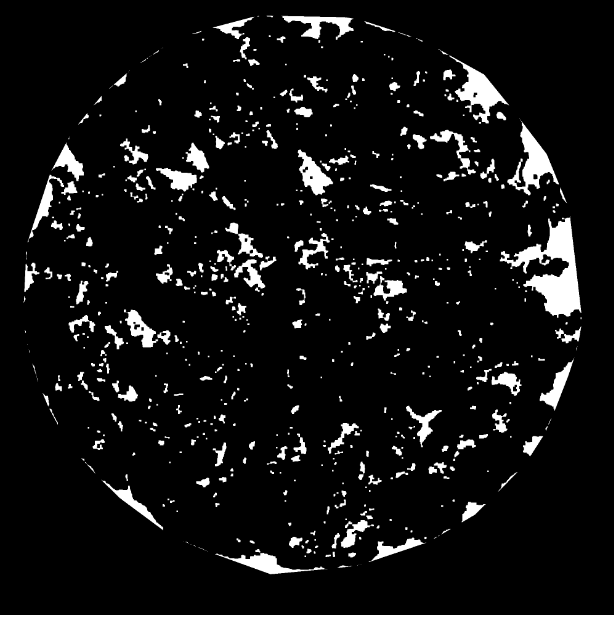
\includegraphics[width=3cm]{fig/seg_final.png}\\
        \scriptsize{Fases da segmentação.}
        \label{fig:metodoMRX}
    \end{figure}
    
\end{frame}

\begin{frame}{Metodologia}{Extração da Região de Interesse.}
    
     \begin{figure}[!htb]
        \centering
        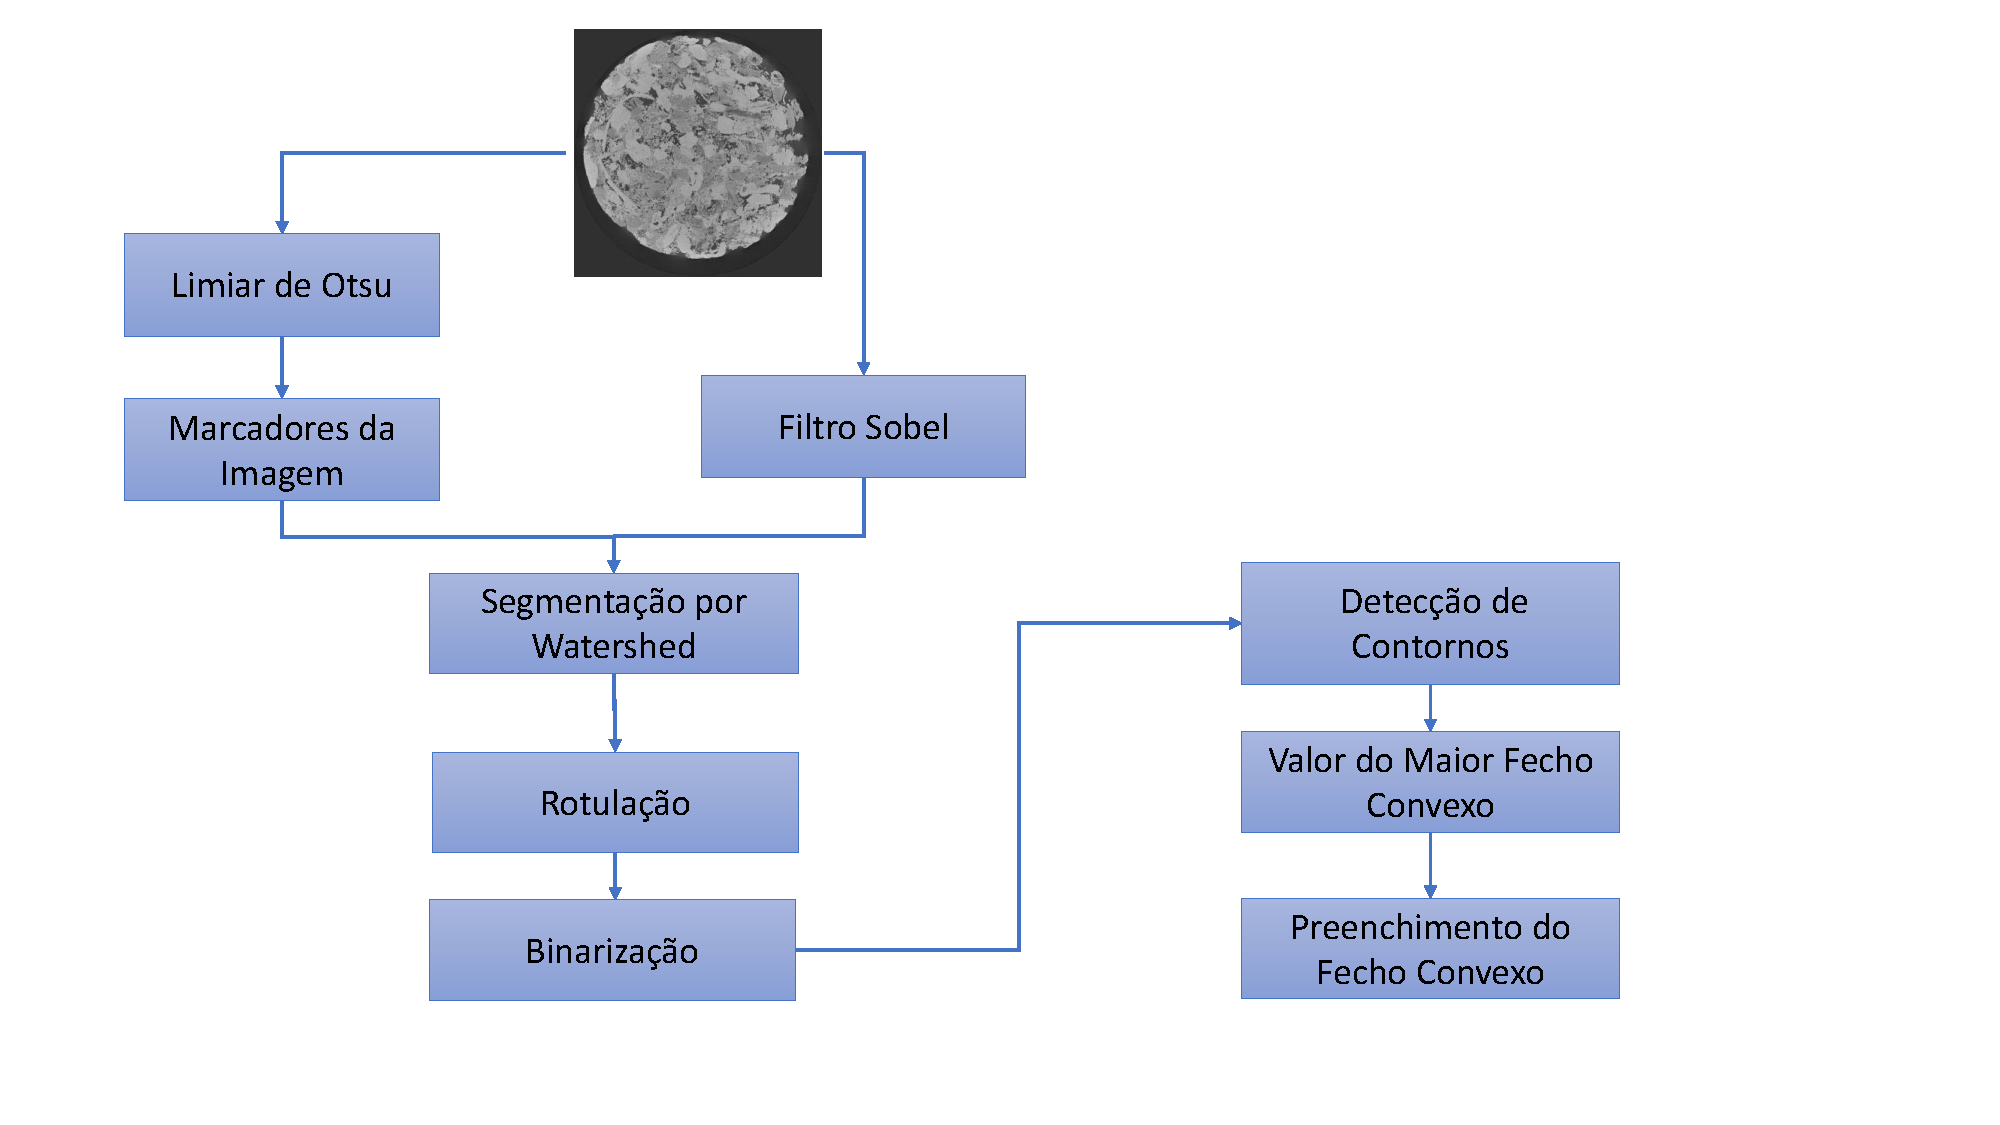
\includegraphics[width=12cm]{fig/mtd-2.pdf}\\
        \scriptsize{Diagrama da metodologia para análise de estruturas de rochas.}
        \label{fig:metodoMRX}
    \end{figure}
    
\end{frame}

\begin{frame}{Metodologia}{Fecho convexo}
    \begin{figure}[!htb]
        \centering
        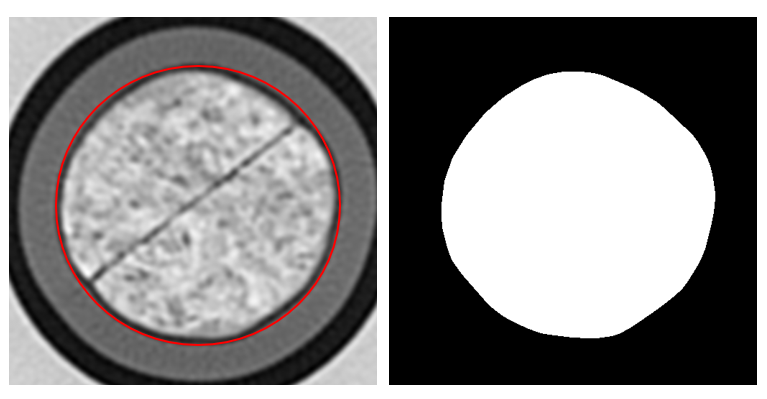
\includegraphics[width=8cm]{fig/ct-sample.png}\\
        \scriptsize{Representação do fecho convexo de interesse e da imagem resultante de sua segmentação.}
        \label{fig:metodoMRX}
    \end{figure}
\end{frame}


\begin{frame}{Metodologia}{Extração das Características das Fraturas}
    O principal passo após a segmentação, neste caso, é a aplicação de técnicas de morfologia matemática que permitam o realce das fraturas.
    \begin{itemize}
        \item \textbf{Operações de Dilatação e Fechamento}
    \end{itemize}
    
    \begin{figure}[!htb]
        \centering
        \subfloat[]{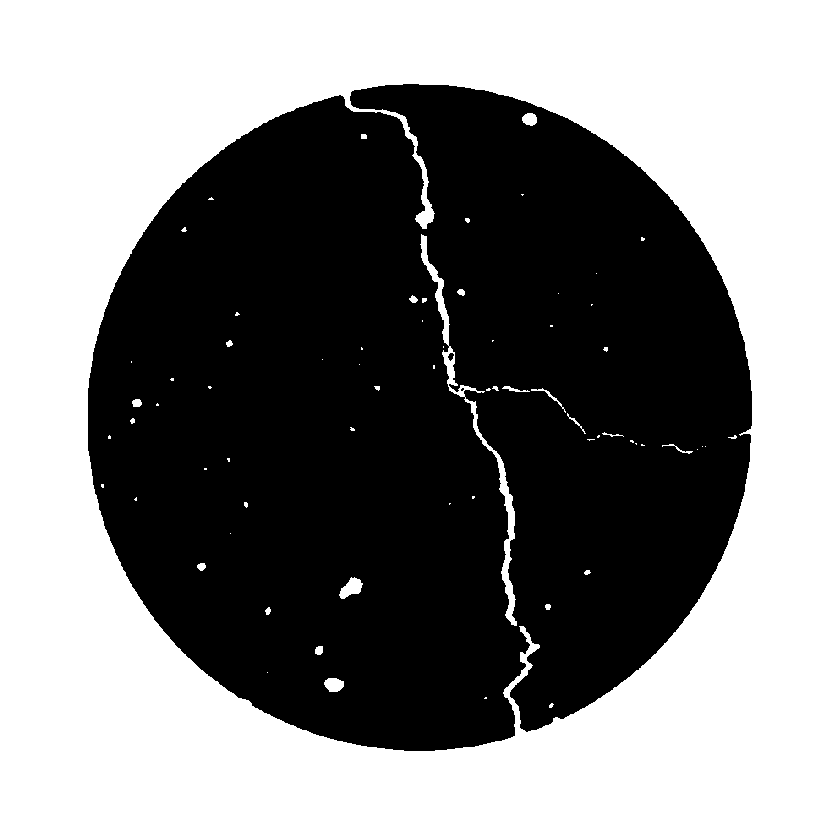
\includegraphics[height=4.0cm]{fig/fratura-thresh.png}} \hspace*{0.2cm}
        \subfloat[]{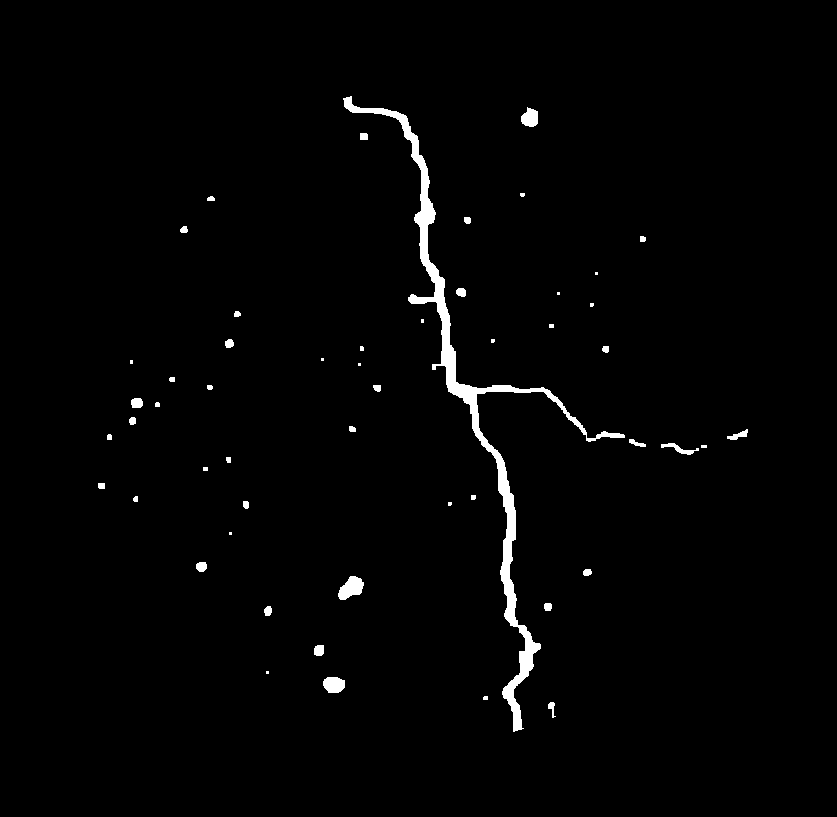
\includegraphics[height=4.0cm]{fig/fratura-seg.png}}\\
        \scriptsize{Pós-processamento da segmentação. (a) imagem segmentada pelo método de Otsu; (b) complementação da segmentação por operações de morfologia matemática.}
    \end{figure}
\end{frame}

\begin{frame}{Metodologia}{Identificação das Fraturas}

\begin{itemize}
    \item Identificação dos contornos que foram extraídos da imagem original a fim de analisar as suas características.
    \begin{itemize}
        \item Uso da função \texttt{findcontours()} da biblioteca \texttt{OpenCV}, essa função auxilia retornando uma lista que contém as descrições de cada estrutura detectada na imagem.
    \end{itemize}
    \item Identificar se os contornos extraídos podem ser classificados como retas.
    \begin{itemize}
        \item Transformada de Hough.
        \item É considerado uma fratura quando se atinge um limiar mínimo de pontos na reta detectada, impedindo que microestruturas sejam extraídas .
    \end{itemize}
\end{itemize}
    
\end{frame}

\begin{frame}{Metodologia}{Angulação}
A angulação é calculada por meio da equação da distância entre dois pontos  $(x_1,y_1)$ e $(x_2,y_2)$ da reta detectada.

\begin{figure}[!htb]
    \centering
    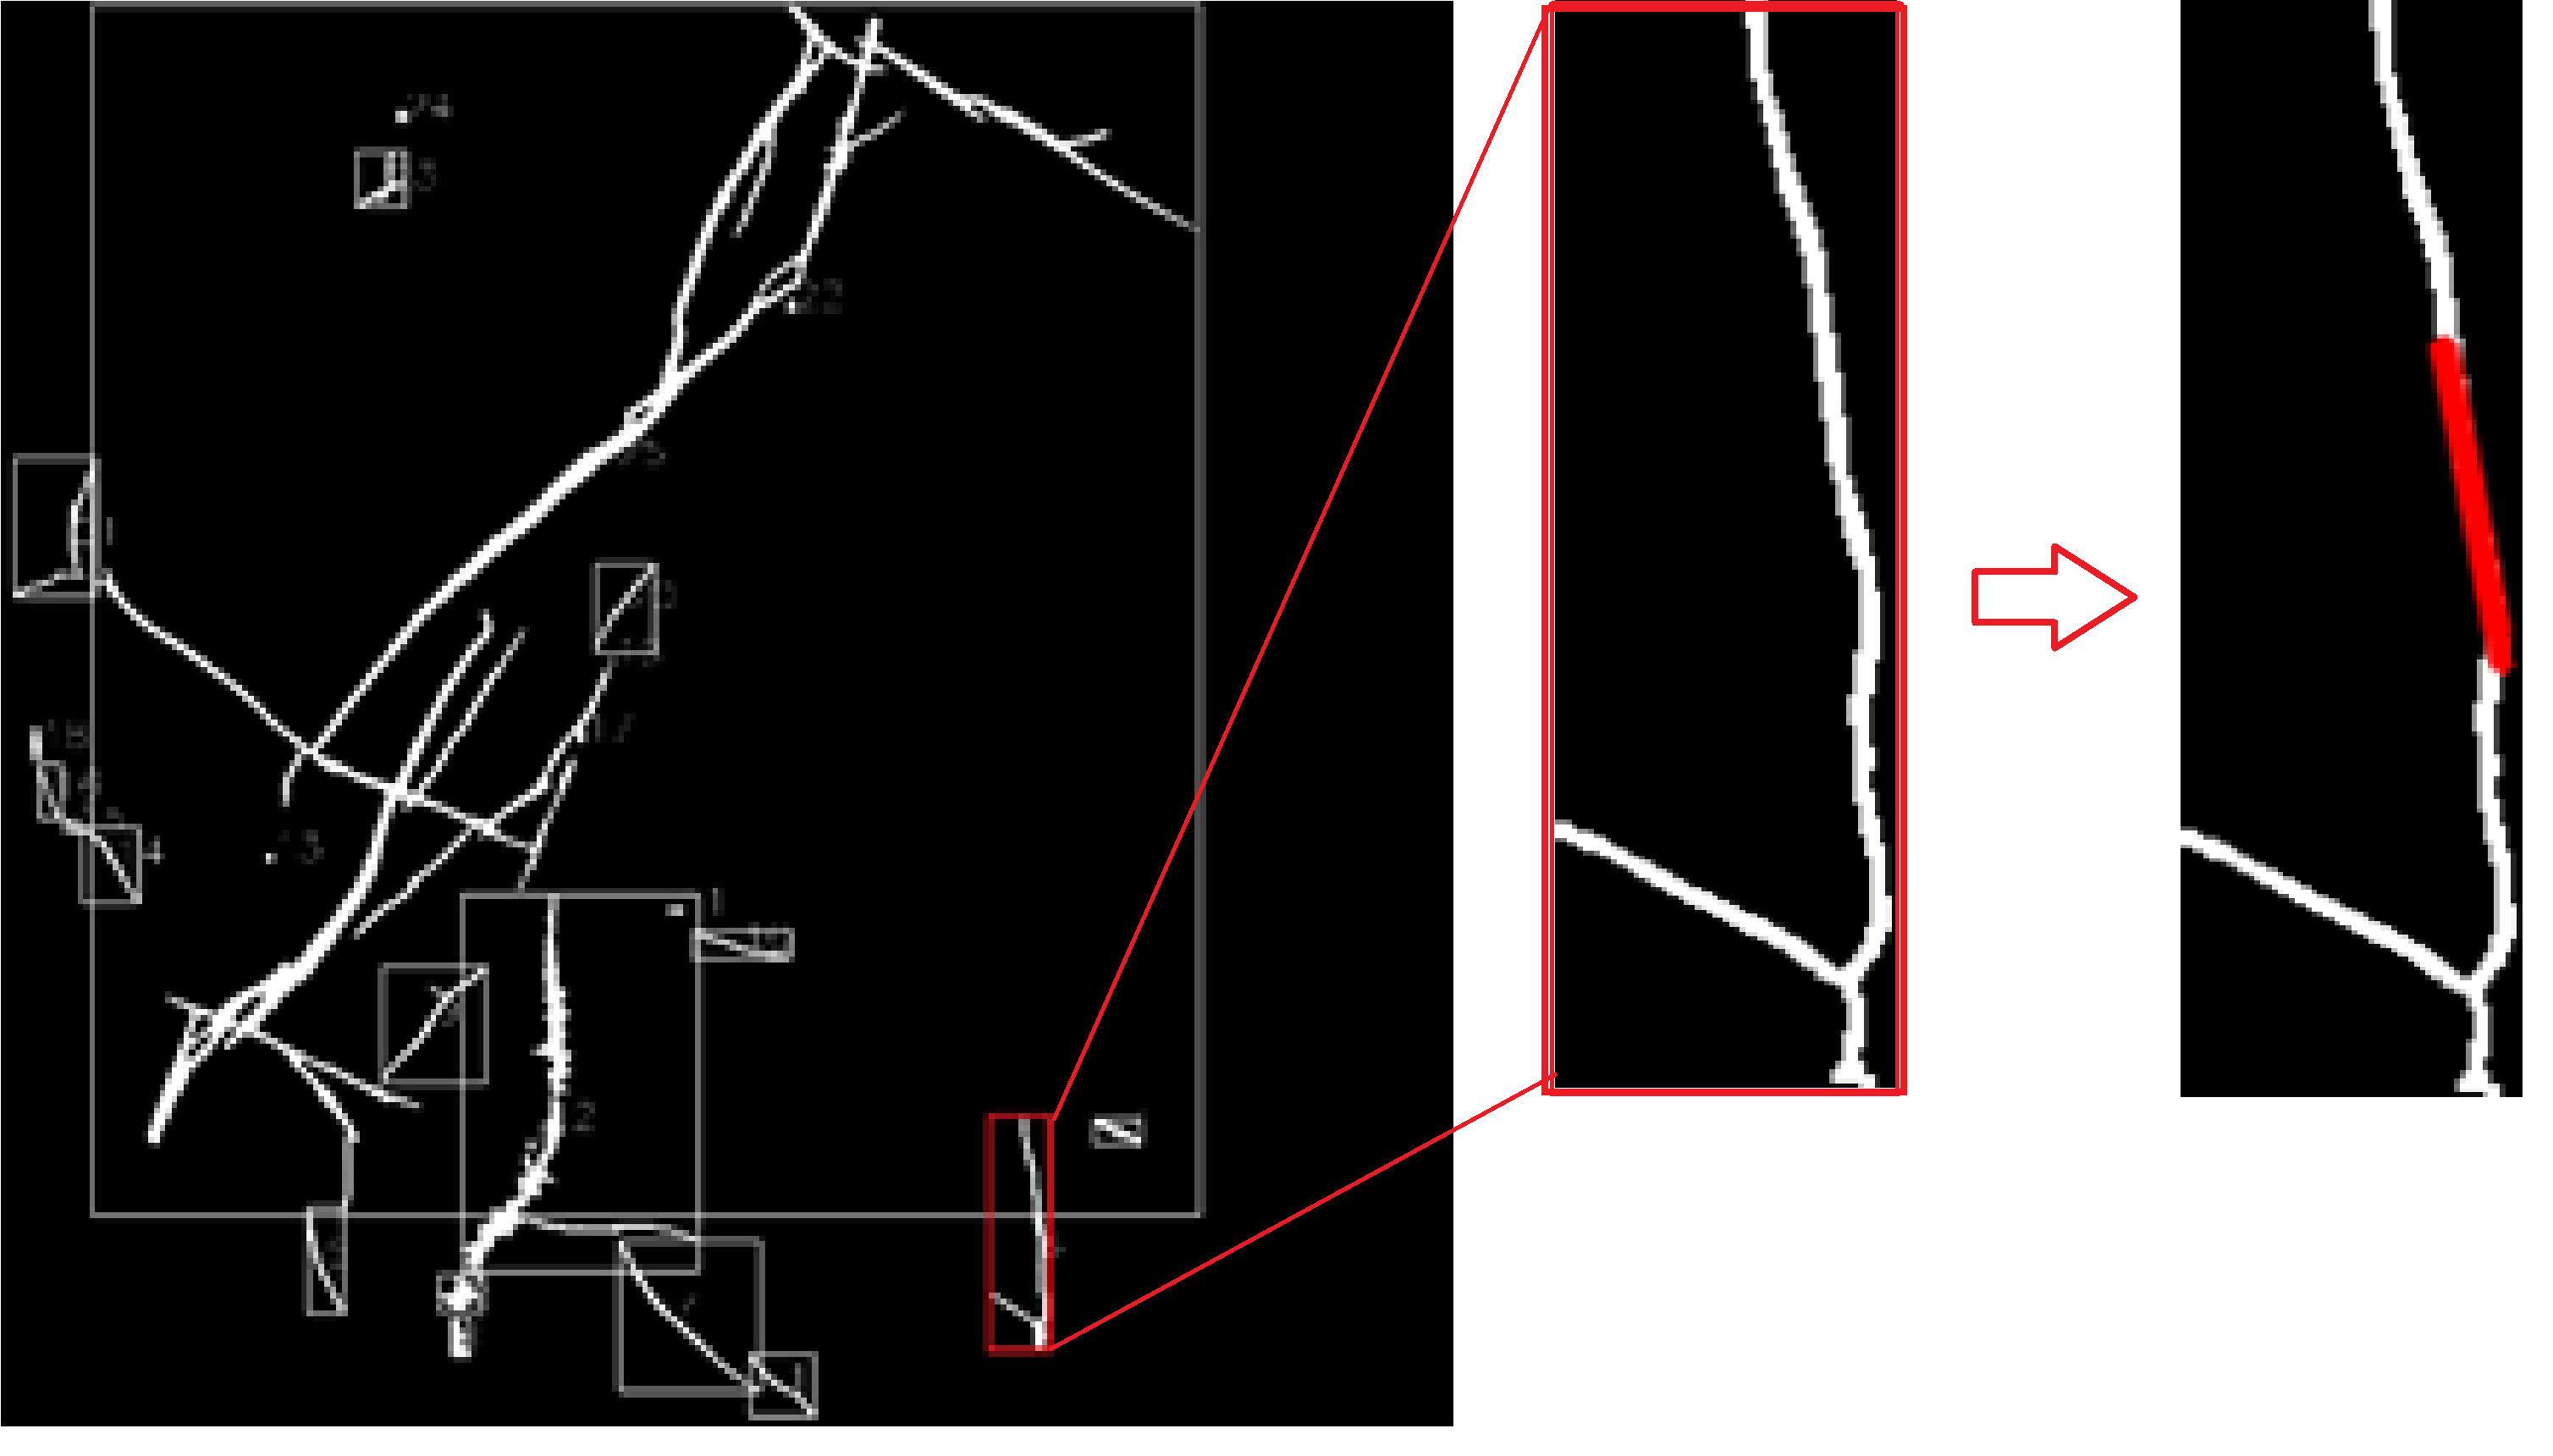
\includegraphics[width=8.5cm]{fig/hough_lines.png}\\
    \scriptsize{Detecção de linhas pela transformada de Hough.}
\end{figure}
    
\end{frame}

\begin{frame}{Metodologia}{Tamanho}

As medidas com respeito ao tamanho são calculadas através dos valores obtidos pelo retângulo envolvente rotativo dos contornos.

\begin{figure}[!htb]
\centering
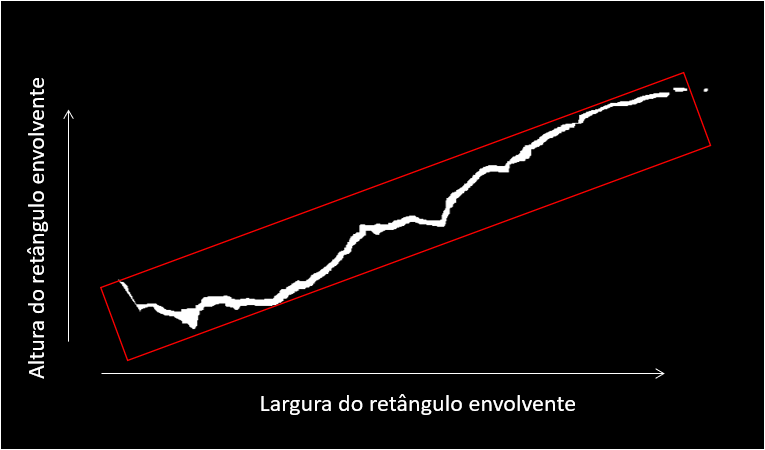
\includegraphics[width=8.0cm]{fig/shape_fracture.PNG}\\
\scriptsize{Ilustração das medidas do retângulo envolvente em relação à fratura.}
\end{figure}

Funções do \texttt{OpenCV} auxiliam a extrair informações como altura e largura.
\end{frame}

\begin{frame}{Metodologia}{Densidade}

\begin{itemize}
    \item Para a densidade linear, utilizou-se o número de fraturas pelo diâmetro da amostra de rocha, sendo:
    \begin{equation}
        d_1 = \frac{\textit{número de fraturas}}{\textit{diâmetro}}
    \end{equation}
    
    
    \item Na densidade 2D, o cálculo é efetuado pela média da largura das fraturas dividido pela área total da amostra, sendo:
    \begin{equation}
        d_2 = \frac{\textit{média(largura das fraturas)}}{\textit{área total da amostra}}
    \end{equation}
    
    \item A densidade 3D, que calcula a relação da área das fraturas pela área da amostra, é dado por:
    \begin{equation}
        d_3 = \frac{\textit{área total das fraturas}}{\textit{área total da amostra}}
    \end{equation}
    
\end{itemize}

\end{frame}

\begin{frame}{Metodologia}{Conectividade: Tipo I,II,II}
    
    \begin{itemize}
        \item \textbf{Processo Inicial:}
        \begin{itemize}
            \item Extração da imagem correspondente ao retângulo envolvente.
            \item Varredura das linhas da imagem resultante.
        \end{itemize}
    \end{itemize}
    
    \begin{figure}[!htb]
    \centering
    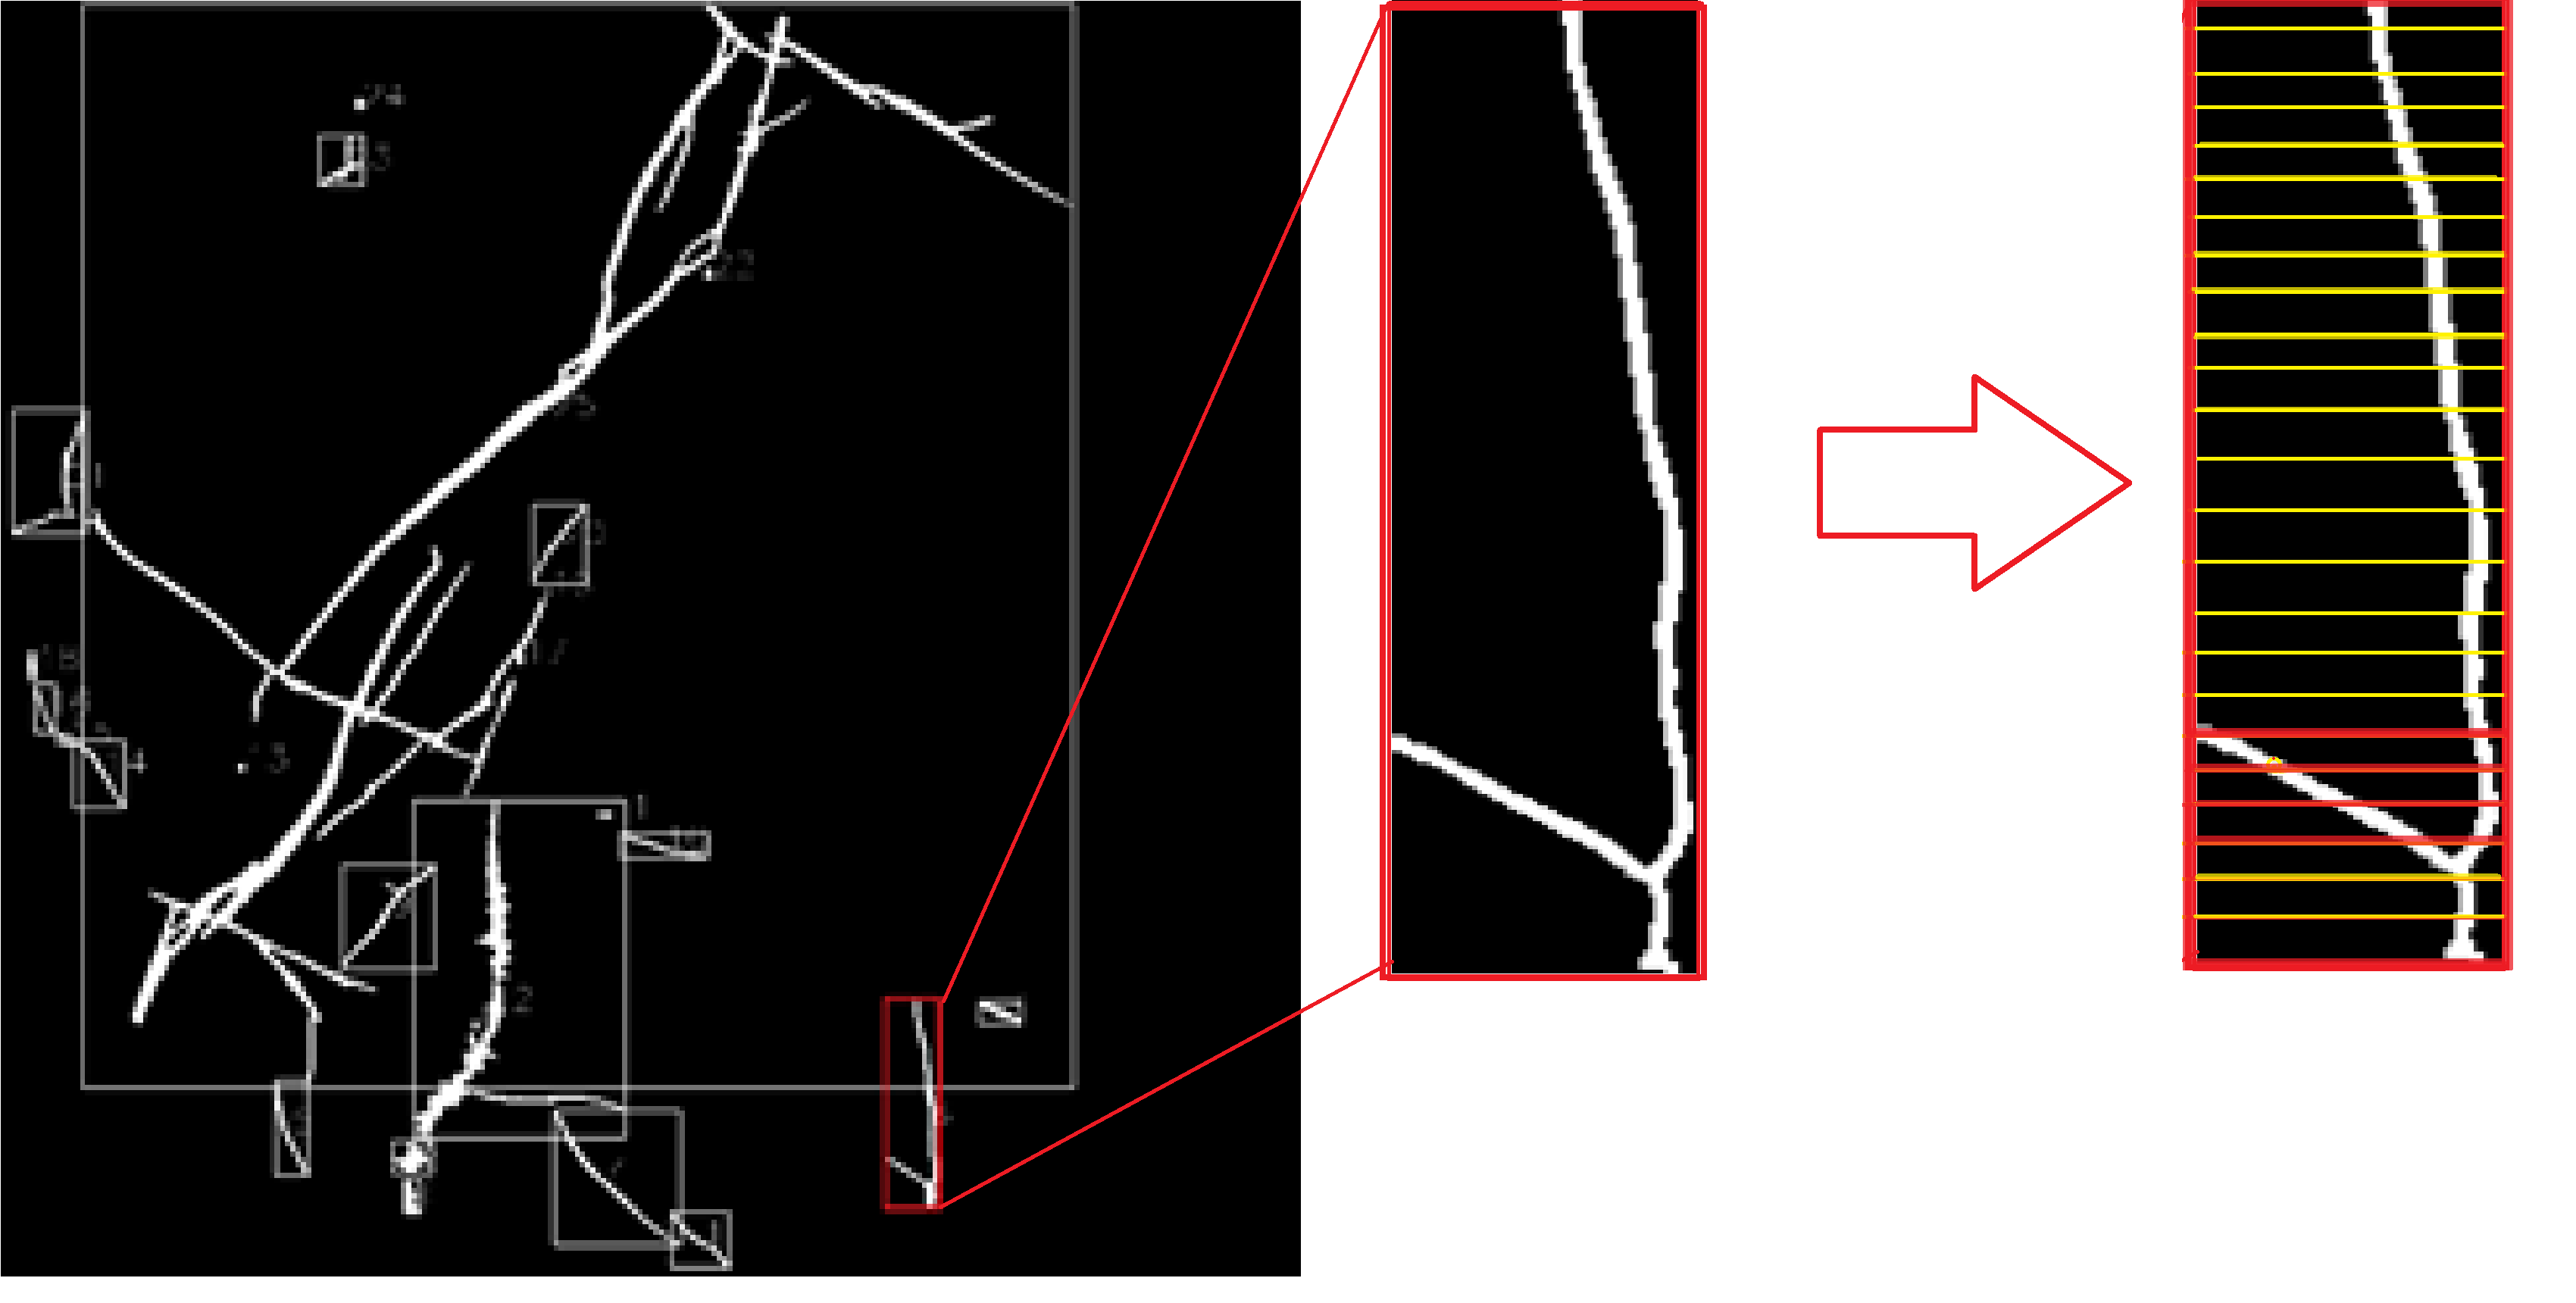
\includegraphics[width=10cm]{fig/conect.png}\\
    \scriptsize{Processo de identificação de bifurcações na fratura.}
    \end{figure}
        

\end{frame}

\begin{frame}{Metodologia}{Conectividade: Tipo I,II,II}
    \begin{itemize}
        \item \textbf{Processo Secundário:}
        \begin{itemize}
        \item Aplicação do método de componentes conexos.
        \item Varredura das linhas da imagem resultante.
    \end{itemize}
    \end{itemize}
    
    
    \begin{figure}[!htb]
    \centering
    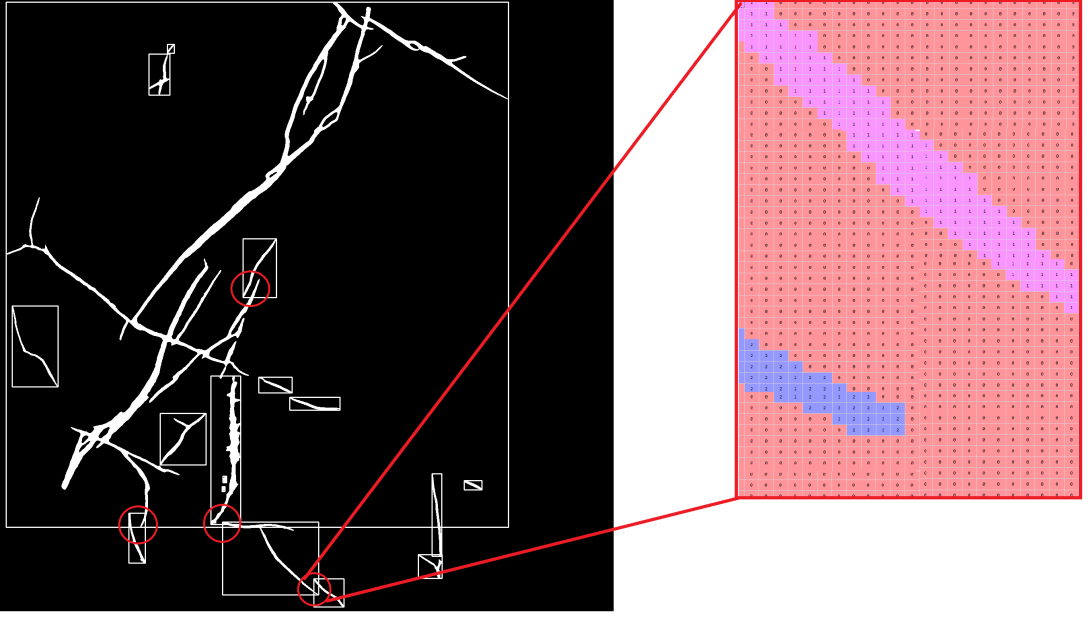
\includegraphics[width=8cm]{fig/conectividade.png}\\
    \scriptsize{Identificação de componentes externos no retângulo envolvente de uma fratura.}
    \label{fig:conectividade}
    \end{figure}

\end{frame}


\begin{frame}{Metodologia}{Conectividade: Sistemática x Não Sistemática}
\begin{itemize}
    \item Análise do padrão das fraturas sistemáticas.
       \begin{itemize}
           \item Segmentação com maior tolerância a ruídos afim de capturar o comportamento da fraturas menores.
       \end{itemize}
   
\end{itemize}    

\begin{figure}[!htb]
\centering
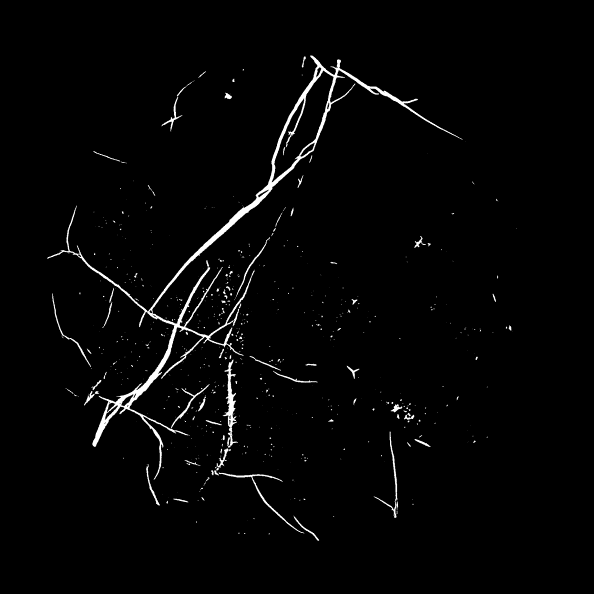
\includegraphics[width=4.5cm]{fig/seg_ruidos.png}\\
\scriptsize{Imagem segmentada com maior tolerância a ruídos.}
\end{figure}

\end{frame}    
\end{document}